\documentclass{llncs}

%\usepackage{llncsdoc}

%\usepackage{makeidx}  % allows for indexgeneration
\usepackage{graphicx}
\usepackage[T1]{fontenc}
\usepackage[english]{babel}
\usepackage[utf8]{inputenc}

\usepackage{paralist}


%%%Math
\usepackage{latexsym}
\usepackage{amsmath}
\usepackage{amssymb}
\usepackage{amsthm}

\usepackage{algorithm}
\usepackage{algorithmic}

\usepackage{longtable}

\usepackage{listings}

\usepackage{color}

\definecolor{darkred}{rgb}{0.5, 0, 0}
\definecolor{violet}{rgb}{1, 0, 1}
\definecolor{green}{rgb}{0.3, 0.95, 0.3}
\definecolor{listinggray}{gray}{0.97}

\lstset{
	basewidth=0.45em,
	backgroundcolor=\color{listinggray},
	basicstyle=\footnotesize\ttfamily,
	breaklines=true,
	keywordstyle=\bfseries,
	stringstyle=\itshape,
	commentstyle=\itshape,
	showspaces=false,
	showtabs=false,
	showstringspaces=false,
	frame=trbl,
	frameround=tttt,
	extendedchars=true,
	numbers=none,
	aboveskip=0.5cm,
	belowskip=0.5cm,
	xleftmargin=0cm,
	xrightmargin=0cm
}


\begin{document}

\title{ONTOSPREAD: Activation of Concepts in Ontologies through the Spreading
Activation algorithm}

\titlerunning{ONTOSPREAD: Activation of concepts in ontologies through the
Spreading Activation algorithm}

\author{Jose Mar\'{i}a \'{A}lvarez\inst{1} \and Diego Berrueta\inst{2} \and Luis Polo
\inst{2} \and Jos\'{e} Emilio Labra\inst{1}} 


\authorrunning{Jose Mar\'{i}a Alvarez et al.}


\tocauthor{Jose Mar\'{i}a \'{A}lvarez, Diego Berrueta, Luis Polo, Jos\'{e} Emilio
Labra} 


\institute{WESO RG, Universidad de Oviedo, Oviedo, Asturias, Spain,\\
\email{\{josem.alvarez,jelabra\}@weso.es},\\ 
 WWW home page: \texttt{http://www.weso.es}
\and
Fundación CTIC, Gij\'{o}n, Asturias, Spain,\\
\email{\{diego.berrueta,luis.polo\}@fundacionctic.org},\\ 
 WWW home page: \texttt{http://www.fundacionctic.org}
}

\maketitle

\begin{abstract}
The present article introduces the ONTOSPREAD API for the development,
configuration, customization and execution of the Spreading Activation
techniques over semantic networks and more specifically over RDF graphs and ontologies 
arising from the Semantic Web area. These techniques have been used to
the efficient exploration and querying of large and heterogeneous knowledge bases 
based on semantic networks in the Information or Document Retrieval domains. 
ONTOSPREAD implements the double process of activation and spread of concepts in ontologies, implicit
graph structures, applying different restrictions of the original model like weight degradation 
according to the distance or others coming from the extension of these techniques like
the converging paths reward. The main application of Spreading Activation
lies in two different areas of interest to digital libraries: 1) construction of hybrid semantic search engines 2) ranking of
information resources according to an input set of weighted resources. These techniques provide a whole framework to ease
the information access, a common required features in the exploitation
of new and existing digital libraries. Finally, in this work an evaluation methodology and 
an example using the Galen ontology are provided to validate the goodness, the improvement and the capabilities of 
this framework applied to digital libraries.
\end{abstract}

\section{Introduction}
\input{sections/intro}
\section{Background}
In this section, the theoretical model of \textit{SA}~\cite{Collins_Loftus_1975,AndersonTheory} is reviewed to 
illustrate the basic components and the operations performed by SA during their execution, specially
the spread of the activation from a node to their adjacent, see Fig.~\ref{fig:spreading}. 
This model is made up of a conceptual network of nodes connected through relations (conceptual graph). 
Taking into account that nodes represent domain objects or classes and edges relations among them, 
it is possible to establish a semantic network in which SA can be applied. The process performed by the algorithm 
is based on a thorough method to go down the graph using an iterative model. Each iteration is comprised of 
a set of beats, a stepwise method, and the checking of a stop condition. 
Following the different stages of SA are presented and defined:

\begin{figure}[h]
 \centering
    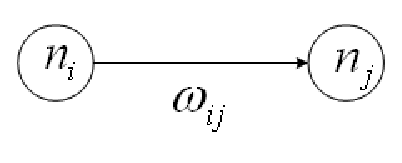
\includegraphics[width=3cm]{images/spreading}
    \caption{Graphical model of \textit{Spreading Activation}}
 \label{fig:spreading}
\end{figure}

\begin{description}
\item [\textit{Preadjustement}:] This is the initial and optional stage. It is usually in charge
of performing some control strategy over the target semantic network.
\medskip

\item [\textit{Spreading}:] This is the spread stage of the algorithm. Concepts
are activated in activation waves. The spreading node activates its neighbor
nodes, see Fig.~\ref{fig:modelo-sa}.
\medskip

The calculation of the activation rank $I_i$ of a node $n_i$ is defined as
follows:

\begin{equation}
I_i  = \sum_j{O_j \omega_{ji}}
\end{equation}
\medskip

$I_i$ is the total inputs of the node $n_i$, $O_j$
is the output of the node $n_j$ connected to $n_i$ and $\omega_{ji}$
is the weight of the relation between $n_j$ and $n_i$. 
If there is not relation between $n_j$ and $n_i$ then
$\omega_{ji} = 0$. 


The activation function $f$ is used to evaluate the ``weight'' of a node and
decide if the concept is active.


\begin{equation}
N_i=f(I_i)=\begin{cases} 0 & \text{if $I_i < \jmath_i$} \\ 1 &
\text{if $I_i > \jmath_i$}
\\ \end{cases}
\end{equation}


$N_i$ is $1$ if the node has been activated or 0 otherwise. 
$\jmath_i$, the threshold activation value for node $i$, depends on the application
and it can change from a node to others. The activation rank $I_i$ of a
node $n_i$ will change while algorithm iterates.

\begin{figure}[h]
 \centering
 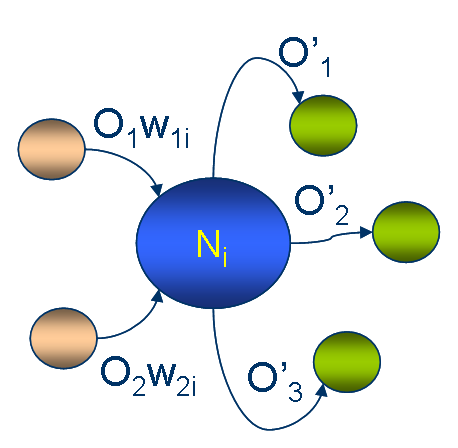
\includegraphics[width=4cm]{images/modelo-sa}
    \caption{Activation of concepts in \textit{Spreading Activation}}
 \label{fig:modelo-sa}
\end{figure}

\item [\textit{Postadjustment}:] This is the final and optional stage. As well as
\textit{Preadjustment} stage, it is used to perform some control strategy in the
set of activated concepts.

\end{description}

\section{Related Work}\label{related-work}
Since SA was introduced by~\cite{Collins_Loftus_1975} in the field of 
psycho linguistics and semantic priming it has been applied to the resolution
of problems trying to simulate the behavior of the brain using a connectionist method
to provide an ``intelligent'' way to retrieve information and data. 

The use of SA was motivated due to the research on graph exploration~\cite{Scott1981}. Nevertheless
the success of this technique is specially relevant to the fields of Document~\cite{turtle91inference} 
and Information Retrieval~\cite{Cohen1987}. It has
been also demonstrated its application to extract correlations between query terms and documents analyzing user 
logs~\cite{Cui03} and to retrieve resources amongst multiple systems~\cite{Schumacher+2008search} 
in which ontologies are used to link and annotate resources.

In recent years and regarding the emerging use of ontologies in the Semantic Web area new applications of SA have
appeared to explore concepts~\cite{Qiu93,Chen95} addressing the two important issues: 1) the selection and 2) the weighting of
additional search terms and to measure conceptual similarity~\cite{gouws-vanrooyen-engelbrecht:2010:CCSR}. 
On the other hand, there are works~\cite{DBLP:journals/cogsr/KatiforiVD10} 
exploring the application of the SA on ontologies in order to create context inference models.The 
semi-automatically extension and refinement of ontologies~\cite{liu_et_al_2005} is other trending topic to apply SA
in combination with other techniques based on natural language processing. Data mining,
more specifically mining socio-semantic networks\cite{paper:troussov:2008}, and applications 
to collaborative filtering (community detection based on tag recommendations, expertise location, etc.) are other 
potential scenarios to apply the SA theory due to the high performance and high scalability of the technique. In particular, 
annotation and tagging~\cite{labraTagging2007} services to gather meta-data~\cite{GelgiVD05} from the Web or to predict social annotation~\cite{Chen:2007:PSA:1780653.1780702} and recommending 
systems based on the combination of ontologies and SA~\cite{citeulike:3779904} are taken advantage of using SA technique. 
Also the semantic search~\cite{conf-sofsem-Suchal08} is a highlight area to apply SA following
hybrid approaches~\cite{bopaEstonia,RochaSA04} or user query expansion~\cite{767402} combining metadata 
and user information.

Although this technique is widely accepted and applied to different fields open implementations\footnote{ 
Texai company~(\url{http://texai.org/}) offers a proprietary implementation of SA.}, are missing. Moreover 
the Apache Mahout~\footnote{\url{http://mahout.apache.org/}} project, a recent scalable machine learning library 
that supports large data sets, does not include an implementation of SA instead of 
providing algorithms for the classification, clustering, pattern mining, 
recommendation and collaborative filtering of resources in which SA should be representative. 
 



\section{ONTOSPREAD API}
%\input{sections/sa}
\section{Evaluation of ONTOSPREAD API}
%\subsection{ONTOPSREAD API in Action}
\section{Conclussions and Future Work}
%\input{sections/conclussions}

% \section{Introduction}
% 
% \textit{Spreading Activation} techniques (hereafter \textit{SA}) rise in the
% Psychology area, as result of human memory researches~\cite{AndersonTheory} and
% more specifically, in the search of ways to exploit human knowledge
% representation:
% \begin{inparaenum} \item Procedural semantics.
% \item Semantic features. \item Semantic Networks\footnote{From Psychology point of
% view.}.\end{inparaenum}
% 
% 
% In the Semantic Web domain and regarding the use of ontologies as knowledge
% bases, they could be taken as a kind of semantic network that models concepts and their relationships using
% a certain sort of logics, e.g. Description Logics (DLs). In some sense,
% ontologies capture a domain knowledge and express it as a logic structure, just
% as the human memory does.
% 
% Knowledge representation using a set of concepts related fits to real world.
% Concepts can express overall relations and data but also particular domain
% knowledge. That's why it is relevant provide an useful method to obtain sets of related
% concepts efficiently and automatically. Usually, the methods to explore knowledge bases can be split into: \begin{inparaenum} efficient search algorithms (based on \textit{Brand and Bounch}) in semantic networks or graphs. \item Neural networks~\cite{Chen95}\end{inparaenum}. \textit{SA}
% techniques provide us a method to explore semantic networks as an iterative way
% (performance oriented) and can be applicable to different problems:
% Information or Document retrieval. Our main goal is applied these techniques to
% ontologies, getting a new method to rank the concepts and their relations
% according to a query.
% 
% \subsection{Related work}
% The use of \textit{SA} as algorithm to explore graphs is not a new approach and
% since 80's\cite{Scott1981} appeared the first works naming it. The
% main use was focused in Document~\cite{Cui03,Kobayashi00,turtle91inference,2917612} and Information
% Retrieval~\cite{Agosti1993,Cohen1987,Baeza99} altough the appearance/born of Internet Spreading
% Activation has been used in retrieve resources from the network:
% hypertext~\cite{Agosti1993} or multimedia with a real trust measurement~\cite{ziegler-lausen-04}. On other hand, these techniques has been used in semantic search based on hybrid approaches~\cite{RochaSA04,XueHYZCM04}, user query expansion~\cite{767402} combining metadata and user information or improve web data annotations~\cite{GelgiVD05}.
% 
% \subsection{Main contribution}
% 
% The aim of this paper is to introduce the application and refining \textit{SA}
% tecniques in the activation of concepts defined in the ontologies and the
% algorithm design through a generic Java API, called OntoSpread that handles the
% process of activation and spread concepts. Furthermore, OntoSpread \footnote{\url{http://sf.net/projects/ontospread}} has
% been developed as an open source project hosts in Sourceforge under LGPL license
% to easy its use and future contributions.
% 
%
% \section{OntoSpread: the design of an API for Spreading Activation}
% 
% Our Spreading Activation API focuses on an open design, best
% practices~\cite{XP,Fowler1999} and makes extensive use of design
% patterns~\cite{Gamma,CoreJ2ee}. We have identified the next basic objects need
% to implement \textit{SA} techniques.
% 
% \begin{itemize}
% 
% \item The \textit{Player} class handles the execution of the algorithm in a
%       stepwise way. This is an application of the \textit{Iterator}
%       design pattern to the activation and spreading processes. The state
%       of the algorithm is captured in a separate class,
%       \textit{OntoSpreadState}, so it is possible to serialize the
%       status and to move backwards.
% 
% \item The \textit{SA} process comprises three sub-processes: \begin{inparaenum} 
%     
%  \item \textit{Preadjustement}: \textit{OntoSpreadPreAdjustment};
%       \item \textit{Spreading} (activation and spreading) with constraints:
% \textit{OntoSpreadRun}; and
%       \item \textit{Postadjustment}:
% \textit{OntoSpreadPostAdjustment}.\end{inparaenum}
% Moreover, the process has information about the knowledge base using a DAO
% pattern so the API is independent from the modelling language. Currently, OWL
% and RDF are supported. Although we have brought forward the use of another
% languages as SKOS-Core or WSML, providing the need operations to extract the
% information about concepts and their relations.
% \end{itemize}
% 
% 
% 
% %\begin{figure}[htb]
% %\centering
% %	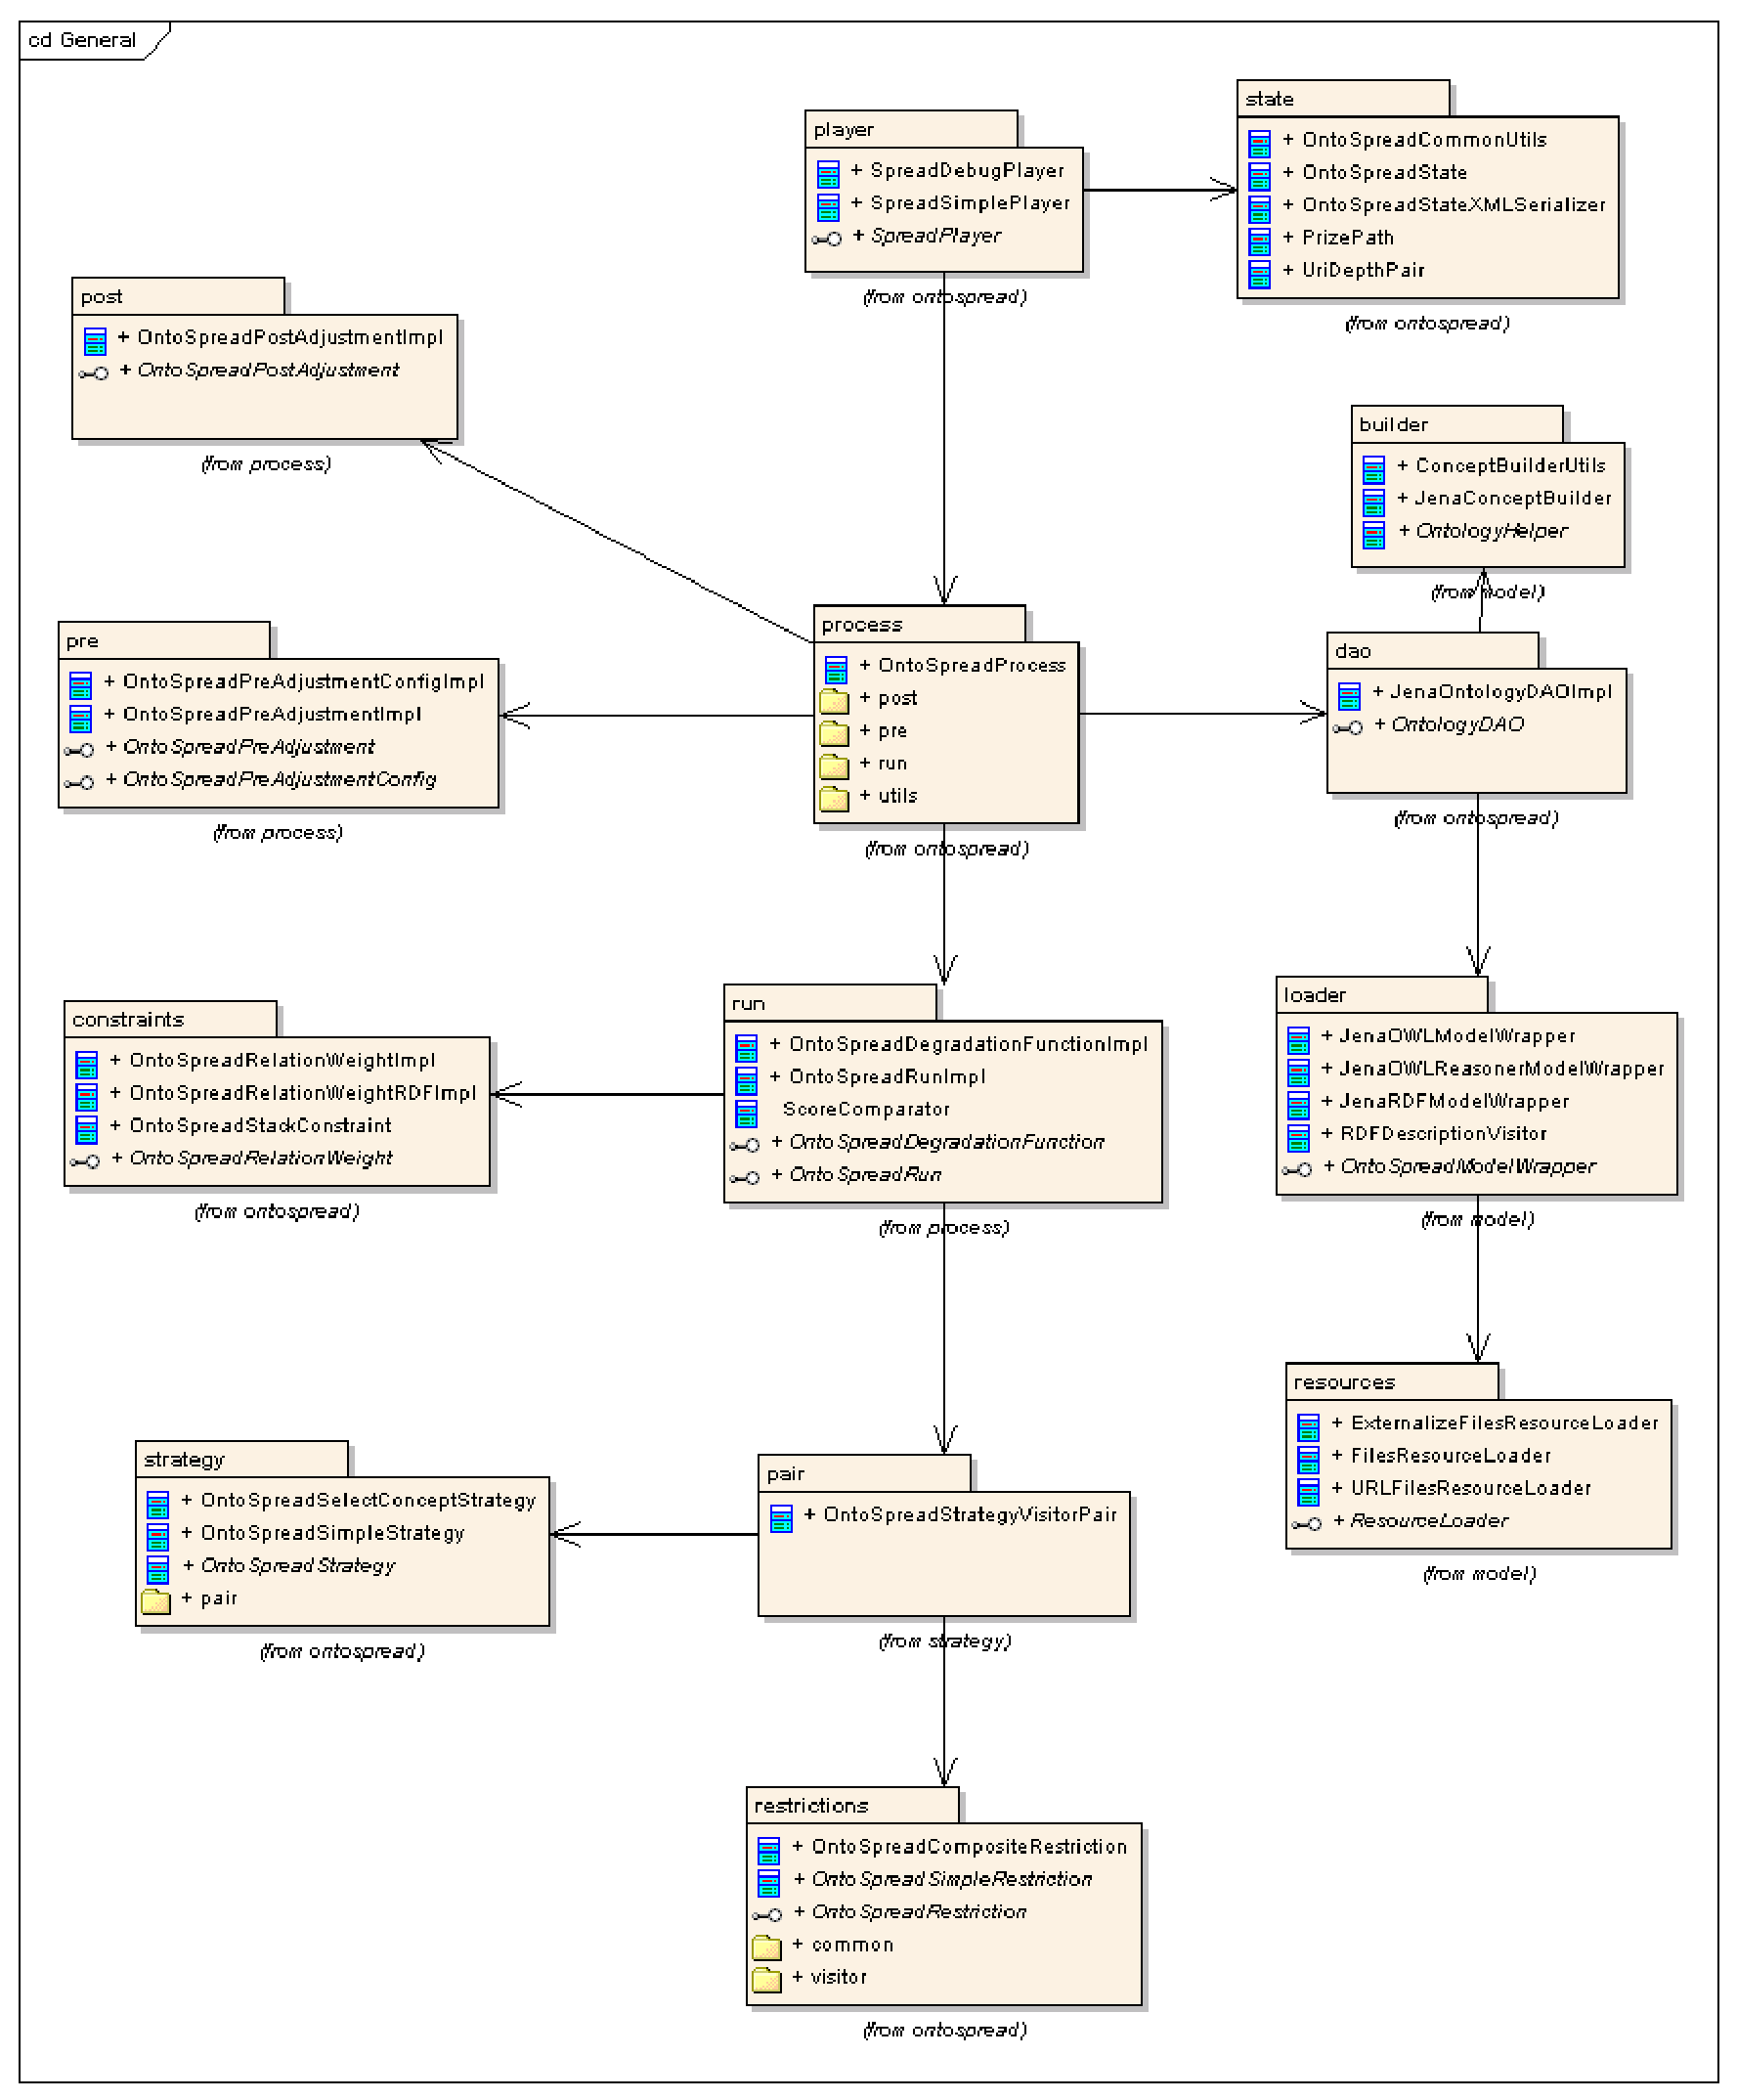
\includegraphics[width=8cm]{diagramas/general}
% %\caption{Diagrama general}
% %\label{fig:diagramas/general}
% %\end{figure}
% 
% 
% \subsection{Designing of the state for \textit{SA}}
% 
% In the first one, the keypoint to design the algorithm falls in how and where
% the information will be available at different iterations. Secondly, we want to
% provide an only one access point to the state of the algorithm trying to avoid
% weak states and providing an easy way for supportting. 
% This object stores the next information: \begin{inparaenum}\item Spread
% concepts. \item Active concepts. \item Paths of activation. \item Concept to be
% spread. 
% \item Generic swap area (to share information). \end{inparaenum}
% 
% \subsection{Designing of restrictions for \textit{SA}}
% The extensibility and flexibility of the algorithm is subjected to a good design
% of the restrictions and the procedure of their evaluation. The next features and design patterns are used to guide the model of restrictions for SA:
% 
% \begin{itemize}
%   \item Any restriction can be considered as a simple restriction and can be
% evaluated to a boolean value.
%   \item Conditions or actions in the algorithm can be composed of several
% restrictions.
%   \item The extension points of  the algorithm, included through a
% \textit{Template Method} design pattern, are strategies to carry out an specific
% action. Each strategy can be subjected to one or several restrictions.
% \item Each restriction can be simple or composed by other ones.
% \textit{Composite} pattern.
%   \item Each action is an strategy. \textit{Strategy} pattern.
%   \item One strategy entails one restriction (or set of them) so the strategy
% seems a client of the \textit{Composite} of restrictions.
%   \item The evaluation of the restrictions to get their value (boolean) is
% carried out
%   through a \textit{Visitor} pattern that fits perfectly to do the evaluation of
% composite objects.
%   \item The evaluation process consists on:
%   \begin{inparaenum}
%   \item Apply the strategy, this step modifies thc execution and reporting
% of batch tests. It provides a framework to configure, combine and load several
% configurations for \textit{SA} and obtain results. We have designed a XML
% vocabulary using XML-Schema and the \textit{Extensible Content Model} xml design
% pattern to build the configuration of the \textit{SA} process. The designing of
% this vocabulary is oriented to be used with JAXB, this technology allow us the
% generation of Java classes automatically and we can marshalling and
% unmarshalling objects providing a good way to configure, load and serialize
% different configurations. The main goal to define a new XML vocabulary can be
% arguable, but this vocabulary is not a new XML to be interchanged among
% applications, we only use inside OntoSpreadTest and to provie state of the algorithm. 
%   \item Validate the changes, the restricctions assert the
% changes.\end{inparaenum}
% 
% \end{itemize}
% 
% 
% 
% %\begin{figure}[htb]
% %\centering
% %	\includegraphics[width=8cm]{diagramas/restricciones}
% %\caption{Diagrama general de restricciones \textit{SA}}
% %\label{fig:diagramas/restricciones}
% %\end{figure}
% 
% 
% \subsection{OntoSpread development}
% 
% The development of the API has been carried out using Semantic Web tecnologies
% and web development tecnology as: Java programming language, 
% Jena\footnote{\url{http://jena.sf.net}} API, 
% JAXB\footnote{\url{
% http://java.sun.com/developer/technicalArticles/WebServices/jaxb/}}, 
% Maven\footnote{\url{http://maven.apache.org}} o
% Spring\footnote{\url{http://www.springframework.org/}}. We have built a
% graphical viewer and debugger,
% \textit{OntoSpread Inspector}, using the graph library
% JpowerGraph\footnote{\url{http://jpowergraph.sf.net}} and
% SWT\footnote{\url{http://www.eclipse.org/swt/}}.
% 
% \subsubsection{Source code metrics}
% 
% We have extracted, using Eclipse\footnote{\url{http://www.eclipse.org}} and the
% metrics plugin\footnote{\url{http://metrics.sf.net/}},  
% some source code metrics (only for OntoSpread API) to show and mesaure its
% quality. We present the most meaningful source code metrics, 
% see Table \ref{tabla:metricas-valores}, based on the definitions
% in~\cite{229953}. These metrics measures cohesion and coupling of the software and can be useful
% to decide if the code is well structured.
% 
%    \begin{longtable}{|p{1cm}|p{4cm}|p{1cm}|p{1cm}|p{1cm}|p{1cm}|p{1.5cm}|}
%         
%         \caption{Source Code Metrics} \label{tabla:metricas-valores}\\
%         \hline
%         \multicolumn{7}{|c|}{\textbf{Source Code Metrics}}\\
%         \hline
%         \textit{ID} &  \textit{Def.} &  \textit{Total} &  \textit{Avg.}& 
% \textit{Std. Dev.} & \textit{Max}& \textit{Scope} \\ \hline
%         \endfirsthead
%         \caption[]{Source Code Metrics (continue)}\\
%         \hline
%         \multicolumn{7}{|c|}{\textbf{Source Code Metrics}}\\
%         \hline
%         \textit{ID} & \textit{Def} & \textit{Total} &  \textit{Avg.}& 
% \textit{Std.
%         Dev.} & \textit{Max}& \textit{Scope} \\ \hline
%         \endhead
%         \hline
%         \multicolumn{7}{|c|}{Continue $\ldots$}\\
%         \hline
%         \endfoot
%         \hline
%         \endlastfoot
% 		TLOC&Total Lines of Code.&5272&&&& \\ \hline
%     		CA&Afferent Coupling.&&$6.524$&$10.545$&48&Package.\\ \hline
% 		RMD&Normalized Distance, $|RMA + RMI - 1 |$.&&$0.32$&$0.347$&1&Package. \\ \hline
% 		NOM&&$0.065$&$0.296$&3&Type. \\ \hline 
% 		RMI&Instability: $CE / (CA + CE)$&&$0.567$&$0.387$&1&Package. \\ \hline
% 		%NOF&Number of Atributtes.&147&$1.256$&$2.039$&12&Type. \\ \hline
% 		%NOP&Number of Packages.&42&&&& \\ \hline
% 		%MLOC&Method Lines of Code.&2661&$4.05$&$6.179$&88&Method. \\ \hline
% 		%WMC&Weighted methods per Class.&852&$7.282$&$6.859$&42&Type. \\ \hline
% 		%NORM&Number of Overriden Methods (no ``Object'' methods).&20&$0.171$&$0.419$&2&Type. \\ \hline
% 		%NSF&Number of Static Attributes.&58&$0.496$&$0.622$&$3$&Type. \\ \hline
% 		NBD&Nested Block Depth.&&$1.204$&$0.516$&4&Method. \\ \hline
% 		%NOM&Number of Methods.&594&$5.077$&$5.297$&33&Type.\\	\hline 
% 		LCOM&Lack of Cohesion of Methods (\textit{Henderson-Sellers}).&&$0.18$&$0.289$&$0.957$&Type.\\ \hline 
% 		VG&McCabe Cyclomatic Complexity.&&$1.297$&$0.735$&6&Method. \\ \hline
% 		RMA&Abstractness.&&$0.113$&$0.186$&0.667&Package. \\ \hline
% 		%NOI&Number of Interfaces.&11&$0.262$&$0.537$&2&Package. \\ \hline
% 		CE&Efferent Coupling.&&$1.976$&$1.282$&5&Package. \\ \hline
% 		%NC&11&$0.094$&$0.539$&5&N/A&Media y máximo por tipo. \\ \hline
% 		DIT&Depth of Inheritance Tree.&&$1.607$&$0.915$&4&Type. \\ \hline
%     	 \hline
%         \end{longtable}      
% 
% 
% All of these values are in the default range defined in the plugin thus we can
% assure the quality of the source code with the desired feautures of \textit{high
% cohesion} and \textit{low coupling}.
% 		
% 
% \subsection{OntoSpread tools}
% 
% The development of a new API requires a test bed to ensure: \begin{inparaenum} 
% \item the functional requirements of the API, we must check if the algorithm
% implements the \textit{SA} model. Black box tests. \item White Box tests, we
% have made 50 unit tests.
%                                                             \end{inparaenum} 
% However, these tests are programmer oriented and we want to provide tools that
% can be used to test the API with nontechnical people. Therefore, we have
% designed and implemented two different tools:
% \begin{description}
% 
%  \item [OntoSpreadTest.] it is a tool for the automatic execution and reporting
% of batch tests. It provides a framework to configure, combine and load several
% configurations for \textit{SA} and obtain results. We have designed a XML
% vocabulary using XML-Schema and the \textit{Extensible Content Model} xml design
% pattern to build the configuration of the \textit{SA} process. The designing of
% this vocabulary is oriented to be used with JAXB, this technology allow us the
% generation of Java classes automatically and we can marshalling and
% unmarshalling objects providing a good way to configure, load and serialize
% different configurations. The main goal to define a new XML vocabulary can be
% arguable, but this vocabulary is not a new XML to be interchanged among
% applications, we only use inside OntoSpreadTest and to provide an easy way to
% handle XML configurations in Java through JAXB. E.g. the XML vocabulary belong
% us configure restrictions as an iterative model, Fig. \ref{example-iterator}.
% Summarizing, OntoSpreadTest is an interpreter of our XML vocabuluary.
% 
% \begin{figure}
% \lstset{language=XML}
% \begin{lstlisting}
% <restriction xsi:type="activationRestriction">
%  <config>
%    <init>0.3</init>
%    <step>0.1</step>
%    <stop>1</stop>
%  </config>  
% </restriction>
% \end{lstlisting}
% \caption{Configuring a restriction.}
% \label{example-iterator}
% \end{figure}
% 
% \item[OntoSpread Inspector.] It is a graphical debugger,
%  of \textit{SA} algorithm. It follows the idea of an
%  inspector inside an ide and belongs: configure, load, run (one step or stepwise)
%  and view the evolution of the semantic network with the concepts (activated,
%  spread, weights, relations, etc.). The main goal of this tool is provide an
%  environment to debug, inspect and change the state of the algorithm.
% 
% \end{description}
%  
% \subsection{Working with OntoSpread API}
% 
% \subsubsection{BOPA}\label{proyecto:bopa}
% OntoSpread API has been integrated in BOPA~\cite{bopaEstonia} project that is
% one of \textit{Semantic Web Use Cases and Case
% Studies}\footnote{\url{http://www.w3.org/2001/sw/sweo/public/UseCases/CTIC/}}
% collected by W3C.\textit{SA} techniques are used as part of an hybrid search
% process, see Fig~\ref{fig:sa-search}, they are in charge of the subprocess of
% query expansion taking as set of initial concepts the concepts retrieved from
% the user query.
%  \begin{figure}[h]
%  \centering
%     \includegraphics[width=10cm]{images/sa-search}
%     \caption{Applying \textit{Spreading Activation} in BOPA}
%  \label{fig:sa-search}
% \end{figure}
% 
% 
% \subsubsection{DBPedia}
% FIXME
%   
% 
% \section{Conclussions and future work}
% 
% \textit{SA} techniques are a combination of restrictions that provide us a
% method to build a set of ranked concepts from a conceptual network as well as a
% human memory does. The application of \textit{SA} is very suitable for a large
% number of scenarios and use cases providing a method to get ``artificial
% suggestions'' closed to human. If we would have to resume \textit{SA} techniques
% in one word, is \textit{flexibility}.
% 
% \begin{enumerate}
% \item Flexibility, extensibily and modularity.
% \item Several scenerarios and use cases to be applied.
% \item The adjusting and refining of the algorithm is a task for domain experts.
% \item It is similar to  a ``helper'' (domain expert).
% \end{enumerate}
% 
% The main goal to improve an algorithm so many flexible as \textit{SA} will be
% adjust and refine its 
% operation for the problem of activation and spread concetps in ontologies. The
% keypoints could be:
% \begin{itemize}
%  \item An automatic learning algorithm to build configurations for OntoSpread
% according to ontologies. Thus, the training of this algorithm could generates
% the best configuration for a specific domain. The algorithm could optimize all
% of the parameters in the algorithm: weights of the relations, activation
% function (parameter of degradation) or the combine of restrictions.
% \item Use of mesaures related to instances~\cite{RochaSA04} as `Cluster
% Measure'', ``Specifity Measure'' or both in the process of activation/spreading.
% \item Development of techniques to select\footnote{Currently, we use ``first
% better''.} the next concept to be spread based on metaheuristics or Tabu
% search~\cite{Glover1990,Gendreau}.
% \item Study and application of \textit{SA} as helper of semi automatic methods
% as mapping~\cite{Bruijin2006} between ontologies or tagging with folksonomies.
% \end{itemize}
% 
% 
%\nocite{*}

% Formal\cite{Scott1981,Cohen1987}
% Data mining\cite{paper:troussov:2008}
% Information Retrieval\cite{SpreadingActivationIR,Helmut2004,Agosti1993,Grinberg:2011:ASA:1940632.1940674}
% Concept exploration\cite{Qiu93} and ontologies\cite{Chen95,DBLP:journals/cogsr/KatiforiVD10,DBLP:journals/ijsc/DixKLVS10,liu_et_al_2005}
% Annotations\cite{GelgiVD05,Chen:2007:PSA:1780653.1780702}
% Tagging\cite{labraTagging2007}
% Web Search\cite{XueHYZCM04}
% Natural Language\cite{Tsatsaronis:2007:WSD:1625275.1625555}
% Recommendations\cite{citeulike:3779904,gouws-vanrooyen-engelbrecht:2010:CCSR}
% Semantic Search\cite{conf-sofsem-Suchal08,Wolverton94retrievingsemantically,Schumacher+2008search,bopaEstonia,RochaSA04,LabraWesoNet}
% Ing. software\cite{CoreJ2EEPatterns}


\bibliographystyle{plain}
% %\bibliographystyle{unsrt}
% %\bibliographystyle{acm}
\bibliography{bib/references}
% \renewcommand{\bibname}{References}
\end{document}
